\articlehead{An Argument for Confomrity}{JM}{2013}

Money does buy happiness.

More specifically, money buys happiness up to around US\$75,000 per year. Beyond that, money has very little effect. (Ref, full text.)

The generally accepted reason behind this phenomenon has nothing to do with money `providing' happiness, rather that a lack of money makes people unhappy. At US\$75,000 pa (and beyond), day to day money problems are essentially nonexistent: when a bill arrives, the bill can be paid.

A 2011 paper, written by Dr Marla Carlson and published in Theatre Journal, ``Furry Cartography'' (full text here), discusses the important of money in the context of the furry community. I originally intended to review her paper as part of my occasional series of ``Furry Research'' articles here on [a][s], but her field can be written about with far more authority by my fellow contributor Quentin Julien (and my recent article reviewing the International Anthropomorphic Research Project, or more specifically the rejoinder by IARP member Nuka, shows how I, as an amateur, can get it wrong).

Briefly then, Dr Carlson talks about the need to earn money, and how (in a capitalist world) ``one must be an individual, but one actualizes that individuality through the purchase of appropriate name-brand products''. She sees furry as a version of this concept. Our `performance' as furries, the way we actualize our furry identity in the real world (perhaps a purchased fursuit or a commissioned work of art) ``fuels the buying and selling of commodities both real and virtual''. Here, she is talking about the furry economy; goods and services sold to help people pursue their furriness.

Furry is personal. It's about identity, or as Dr Carlson puts it: ``for some as an expression of an inner essence and for others as escape from a restrictive human persona''. Yet public and outward displays of our furriness are important. Dr Carlson argues that ``the fandom manages its public image in order to remain edgy but not out of bounds'', which roughly defines the range of expressions we allow within the furry community: the extent to which people can express themselves while still fitting in. So an animal-themed t-shirt in public is okay, whereas `anatomically correct' gear is not.

External expression of identity is important to everyone. People in the mainstream are often flummoxed by expressions from the fringe. Why, they might argue, do gay people need to make such a big deal about their sexuality; why can't they just leave it at home and act `normal' elsewhere? The answer, of course, is that people in the mainstream also express themselves, just that they are lucky enough to conform to society's norms without having to make any special effort.

(As an aside, this blind spot is known as majority privilege. To choose another convenient example: the subset of gamers that get fired up whenever someone points out that women aren't fairly represented in the gaming mainstream—these guys are used to games being male-dominated, so anything challenging this feels like it's pandering to others, so they complain that they're being marginalized. See also: straight people who begrudge redefinition of the word `gay'.)

It's sometimes difficult to express furriness in a public space. Furry spaces such as conventions, private parties, and corners of the online world, are environments where we can express ourselves without having to worry about conforming to the mainstream. Furry spaces can act as important relief valves: they allow us to vent the pressure of acting `normal' (or `normal enough') in the wider world. We understand that we may need to mask our furry selves in some circumstances: maybe at work, or around extended family.

Some furries, of course, manage to `opt out' from the requirement for conformity by largely excusing themselves from society. Many of us fantasize about this (just read Rabbit's dreamy `what if' article from a few weeks ago, speculating on the founding of a furry town). A typical fantasy involves a big rural space away from other people, an idea that probably requires a big chunk of cash, to say nothing of the psychological challenges of isolation. For most of us, the fantasy will remain a pipedream.

For those of us who can't escape, there is a balance to be struck. The need for personal expression must be tempered with the requirement to meet society's norms. An external expression of identity that fails to meet mainstream standards can be costly: wearing a collar will probably harm your chances of getting that office job.

The way you present yourself affects how people react to you. If you fit in, people are more open, lowering the barrier for a social interaction. People are more likely to engage with someone who doesn't scare the horses, so to speak.

(There is also a phenomenon called the spotlight effect, familiar to anyone who has found themselves underdressed for a social gathering. Most people become anxious when they feel like they are presenting themselves in an inappropriate fashion. This social pressure is often more about self-perception than about the others: it's also felt by transgender people trying to `pass' for the first time.)

This article, then, is an argument for the value of meeting the expectations of mainstream society. This article is an argument for conformity.

I argue for conformity of appearance, not conformity of thought. The two are often confused. The sight of identically-dressed commuters is often derided, as if all commuters were mindless automatons, as suggested by pejorative terms like rat race. But nothing is further from the truth: each commuter has a personal identity, one that is not on display. A furry in a business suit is still a furry, just one in a different costume.

\begin{figure}
  \begin{center}
    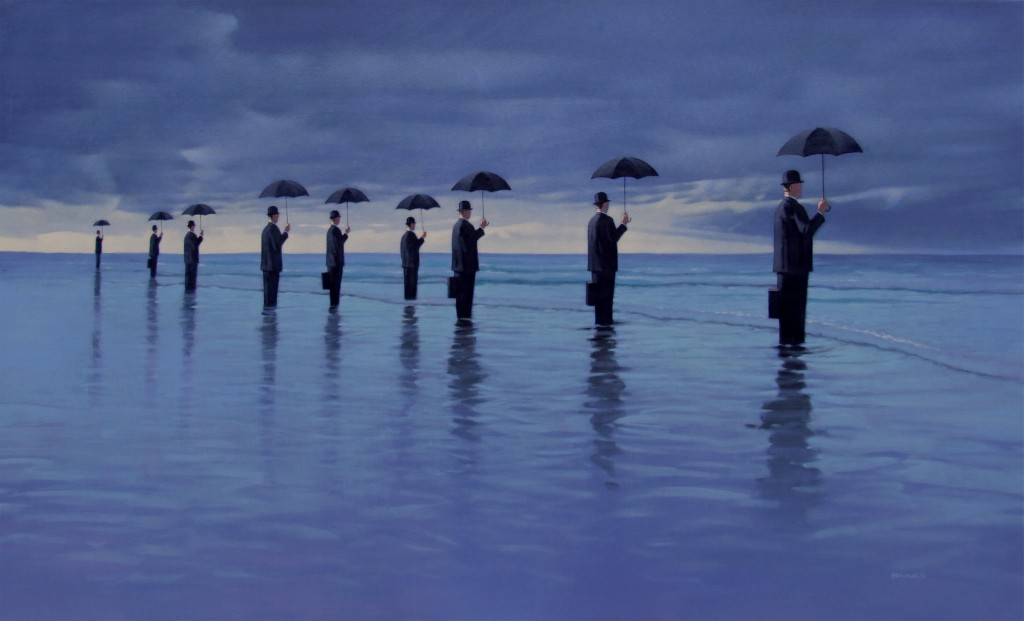
\includegraphics[width=\textwidth]{content/assets/conformity--escape}
  \end{center}
  \caption{This is an Andrew Baines painting, ``Escape of the Corporate Battery Hen''. They look like furries, fetishists, and deviants to me. You can buy it at www.andrewbaines.com/prints.html}
\end{figure}

I believe that meeting society's norms—conforming—increases personal happiness. It's a compromise, and the requirement to moderate external expressions of identity can be challenging. But the reward is a better, broader, happier life.

Someone who puts on a good `normal suit' will be less constrained by the wider world. A good `normal suit' doesn't mean you are normal. It simply means that you restrict what you show to the outside world. Most people would argue that it's a bad idea to share teenage sexual exploits in a public forum—Facebook, say—because they may linger on the internet to be discovered by future employers, lovers, or family members. Someone who refrains from sharing details of a raucous 18th birthday is simply keeping their `normal suit' on.

Those furries who are meeting society's expectations are giving themselves more opportunity in life. They are likely to earn more money, be freer to travel, and have more options to express themselves as furries. To put it another way: would you rather wear a collar to a job interview in 2013, or a fursuit to Eurofurence in 2015?

It's not very romantic to suggest that the best path is through engaging with the mainstream; through moderating one's appearance, through earning and spending money, through ignoring the philosophical messages of Rage Against The Machine. It's especially distasteful if you, like many furries (including me), are most at home in the fringes of society.

The argument for conformity is a pragmatic one. It's about balancing an individual interior with an acceptably bland exterior. It's about, on one hand, working within society's constraints and, on the other, finding appropriate outlets for self-expression.

Andrew Baines says that conformists ``head off to work nine to five every day and they'll do this until they turn 60 and then they'll probably get a gold watch and drop dead``. I think this is false. Instead, I think they experience the relief and benefits of conformity, and never look back.
